\chapter{フリードマン力学と状態方程式}

\lectureoverview{一様な膨張は局所的な束縛系の物理から分離されねばならず、内在的幾何は埋め込みの形状から分離されねばならない。これらの区別が確立されれば、宇宙原理は時空計量を1つのスケール因子\(a(t)\)と1つの曲率ラベル\(k\)に還元する。するとアインシュタイン方程式の時間-時間成分がフリードマンエネルギー方程式となる。これを解くには依然として圧力とエネルギー密度の物質的関係が必要である。断熱熱力学と状態方程式\(P=w\rho\)から\(\rho\propto a^{-3(1+w)}\)が得られ、物質、放射、真空エネルギーが1つの枠組みに統一される。}

\section{物理的描像を確定する問い}

\subsection{空間は地平線の手前で繰り返し得るか}

有限な平坦宇宙は周期的セルによって表現できる。そのセルが観測可能領域より小さければ、光はそれを横断でき、空には同じ構造の繰り返し像が含まれるであろう。それらの繰り返しを検出することは、単に見慣れた銀河を認識することより難しい。像は異なる方向と時代から到来し、宇宙進化によって変容しているからである。それでもなお、周期的トポロジーには観測可能な帰結がある。

\begin{classroomqa}
\audiencequestion{宇宙全体が観測可能な宇宙より小さいことはあり得るか。}
\lecturerresponse{周期的に同一視されたトーラスが自然な提案である。その場合、我々は同じ物理的領域の繰り返しの複製を観測していることになり、比喩的に言えば裏口から自分自身を見ていることになる。対応する宇宙の周期性の探索は支持する証拠を生み出しておらず、小さな基本セルに制約を課している。この可能性は幾何学的に整合的であるが、すでに観測された領域より小さい宇宙はこの証拠によって支持されていない。\lecturetimestamp{00:01:17--00:02:33}}
\end{classroomqa}

\subsection{膨張は束縛系を引き離さない}

宇宙膨張は、平均的な宇宙幾何における自由に運動する物質の大規模な運動を記述する。すべての固有長が増大しなければならないという普遍的な命令ではない。電磁気力は原子を束縛し、重力は惑星系を束縛し、通常の分子間力は固体を束縛する。これらの相互作用は、そのようなスケールにおける宇宙論的補正より桁違いに強い。

\begin{classroomqa}
\audiencequestion{膨張は暗黒エネルギーによって引き起こされるのか、そしてなぜ原子や惑星軌道は空間とともに膨張しないのか。}
\lecturerresponse{宇宙が膨張することは暗黒エネルギーが発見される前から知られていた。暗黒エネルギーは膨張を加速させることによって変化させるのであり、膨張の定義でも元々の原因でもない。束縛系は局所的な力が支配するためハッブル流に従わない。加速された背景は原子や軌道に極めて小さな摂動を生じ得るが、通常の束縛は系が飛び散ることを許さず、ほとんど変わらない平衡を回復する。\lecturetimestamp{00:02:36--00:06:50}}
\end{classroomqa}

\subsection{時間依存幾何におけるエネルギー}

残る反論は力についてではなく簿記についてである。束縛軌道が小さな宇宙論的摂動に絶えず抵抗するなら、必要なエネルギーはどこから来るのか。この前提は、大域的な時間並進対称性を持たない時空に、静的背景からの保存則を持ち込んでいる。

\begin{classroomqa}
\audiencequestion{局所的な束縛が膨張に抵抗するとき、エネルギーはどこから来るのか。}
\lecturerresponse{静的宇宙におけるエネルギー保存は時間並進不変性から従う。すなわち、実験を時間的にずらしても背景とその法則は同じに見える。膨張する時空はそのような大域的意味での時間並進不変性を持たないため、宇宙全体に対して単一の保存された全エネルギーが存在する必要はない。局所的な応力エネルギーの保存は依然として成り立ち、以下に連続の方程式として現れる。成り立たないのは、幾何が変化する間、大域的に定義された宇宙エネルギーが固定されねばならないという素朴な主張である。\lecturetimestamp{00:06:52--00:09:24}}
\end{classroomqa}

\subsection{一様性は粗視化された命題である}

宇宙原理はスケールに依存する。閉じた部屋の空気は部屋のスケールではほぼ一様であり得るが、分子スケールでは粒状である。宇宙も同様に惑星、銀河、銀河団、密度揺らぎを含む。一様性と等方性は、それらの構造が位置や方向を選ばなくなるほど十分大きな距離にわたる平均的振る舞いを指す。

\begin{classroomqa}
\audiencequestion{小規模な束縛構造は一様性と等方性に矛盾するか。}
\lecturerresponse{しない。厳密な一様性は小規模スケールでは破れている。ちょうど、個々の分子を分解して見れば空気についても破れているのと同じである。数億光年およびそれ以上のスケールでは、観測される分布は近似的に一様であり、方向に依存しない。我々が観測できる領域を超えると、一様性は確立された事実ではなく、その帰結を検証しなければならない仮定にとどまる。\lecturetimestamp{00:09:27--00:10:55}}
\end{classroomqa}

\section{計量の言明としての一様性と等方性}

一様性と等方性は、力学的主張となる前に幾何学的な言明である。アインシュタイン方程式は、幾何学が時間とともにどのように変化するかを教えてくれる。まず、任意の一時点でどのような空間幾何学が許されるかを述べなければならない。

\begin{classroomqa}
\audiencequestion{一様性と等方性は数学的には何を意味するのか。}
\lecturerresponse{空間を計量で記述し、ある一点を中心とする座標\(x^i\)を選ぶ。次に、別の一点を中心とする座標\(y^i\)を選ぶ。一様性とは、計量を同じ関数形のままにして原点を移動させる変換が存在することを意味する。そのとき、すべての点は他のすべての点と幾何学的に等価である。等方性はさらに各点のまわりの回転対称性を加えるので、どの方向も特別ではない。\lecturetimestamp{00:11:13--00:14:26}}
\end{classroomqa}

\begin{definition}
任意の点を他の任意の点へ等長変換で移せるならば、その空間は\emph{一様}である。その点を通る回転がその幾何学を変えないならば、その点について\emph{等方}である。一様かつ等方な空間には、特別な位置も特別な方向もない。
\end{definition}

ユークリッド平面はこの定義を明快にする。デカルト座標では、
\begin{equation}
ds^2=dx_1^2+dx_2^2.
\label{eq:c04-flat-metric}
\end{equation}
原点を定数\(a_1\)および\(a_2\)だけ移動させる。
\begin{equation}
y_1=x_1+a_1,
\qquad
y_2=x_2+a_2.
\label{eq:c04-flat-translation}
\end{equation}
\(dy_i=dx_i\)であるから、平行移動後の計量は
\begin{equation}
ds^2=dy_1^2+dy_2^2.
\end{equation}
点をラベルする記号は変わったが、距離の規則は変わっていない。これが一様性の最も単純な実現である。回転も同様に計量を保つので、平面は等方でもある。

球面がより自明でないのは、その座標がより不便であるからにすぎない。南極を原点として選ぶと、単位二次元球面は
\begin{equation}
d\Omega_2^2=dr^2+\sin^2 r\,d\theta^2.
\label{eq:c04-sphere-metric}
\end{equation}
と書ける。東の極が新しい原点となるように球面を回転させる。座標変換は煩雑であるが、結果は再び式~\eqref{eq:c04-sphere-metric}である。丸い球面上のどの点も幾何学的に区別されない。

\begin{classroomqa}
\audiencequestion{周期的に同一視された平坦なトーラスは一様かつ等方か。}
\lecturerresponse{それは平行移動の下で一様である。周期セル内のどの点も同じ局所幾何学をもつ。しかし完全に等方はない。同一視が特別な周期的方向と長さを選び出すからである。それらの軸の一つに沿って見ることは、一般的な斜めの方向に見ることとは大域的に異なる。したがってトーラスは、完全な等方性を伴わない一様性の明快な例を与える。\lecturetimestamp{00:20:18--00:21:30}}
\end{classroomqa}

観測される大規模な一様性は、我々の地平線内における宇宙原理を動機づける。それを観測可能な領域の外へ拡張することは直接の観測ではなく公準である。我々がその公準を受け入れるのは、それが鋭く定義された幾何学を与え、その帰結をデータと突き合わせられるからである。

\section{内在的幾何学と埋め込み}

空間が球面的と呼ばれるとき、より大きな部屋の中に置かれた風船のゴム表面を想像しがちである。その絵は描く助けにはなるかもしれないが、周囲の部屋は宇宙論的主張の一部ではない。重要な幾何学は\emph{内在的}である。すなわち、空間内にとどまる観測者によって測定できる距離と角度から成る。

\subsection{閉じた一次元世界}

閉じた一次元世界を考える。それを円として、角を丸くした正方形として、あるいはピーナッツ形のループとして描いてもよい。その線に閉じ込められた住人は、線に沿った距離だけを測る。二つのループが同じ全周長をもつならば、その住人たちは、描かれた形がまったく異なって見えても同じ内在的幾何学に出会う。

\begin{figure}[htbp]
\centering
\includegraphics[width=0.72\textwidth]{lecture_04_figure_05.png}
\caption{内在的幾何学を埋め込みの形から区別するために用いられる、丸い閉ループと変形した閉ループ。この後のフレームは、先の議論の際に描かれた図を保持している。関連する内容は00:23:21--00:25:59に現れる。}
\label{fig:c04-intrinsic-board}
\lectureframe{00:59:54.899}
\end{figure}

一次元計量はすべて局所的に平坦である。短いひもの一片は伸ばさずにまっすぐにできるので、周囲の平面内で見える曲がりは内在的曲率ではなく外在的なものである。閉じたループには大域的なモジュラス、すなわちその円周があるが、一次元の住人が測定できる内在的な局所の曲がりはない。

\begin{figure}[htbp]
\centering
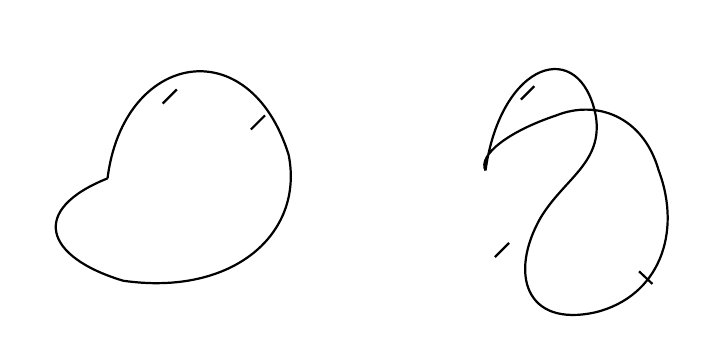
\begin{tikzpicture}[scale=1.0]
\draw[line width=0.8pt] (0,0)
  .. controls (0.2,1.6) and (1.8,1.9) .. (2.3,0.3)
  .. controls (2.5,-0.7) and (1.6,-1.5) .. (0.2,-1.3)
  .. controls (-0.8,-1.0) and (-1.0,-0.4) .. (0,0);
\draw[line width=0.8pt] (0.70,0.95) -- (0.88,1.13);
\draw[line width=0.8pt] (1.82,0.62) -- (2.00,0.80);

\draw[line width=0.8pt] (4.8,0.1)
  .. controls (5.0,1.5) and (6.0,1.8) .. (6.2,0.8)
  .. controls (6.3,0.2) and (5.8,0.0) .. (5.5,-0.5)
  .. controls (5.1,-1.2) and (5.3,-1.9) .. (6.2,-1.7)
  .. controls (7.0,-1.5) and (7.3,-0.7) .. (7.0,0.1)
  .. controls (6.8,0.8) and (6.2,1.0) .. (5.7,0.8)
  .. controls (5.1,0.6) and (4.7,0.3) .. (4.8,0.1);
\draw[line width=0.8pt] (5.25,1.00) -- (5.42,1.17);
\draw[line width=0.8pt] (5.10,-0.82) -- (4.92,-1.00);
\draw[line width=0.8pt] (6.75,-1.18) -- (6.92,-1.34);
\end{tikzpicture}
\caption{円と変形したループの明快な再構成。等しい円周は等しい内在的一次元幾何を意味する。}
\label{fig:c04-intrinsic-redraw}
\end{figure}

\begin{classroomqa}
\audiencequestion{有限な線分も同じ種類の一次元空間だろうか。}
\lecturerresponse{いいえ。線分には二つの端点があるが、閉じたループには端点がない。この位相的区別は内在的であり、どちらの対象をより大きな空間内で曲げても取り除くことはできない。位相が固定されれば、線分はその長さによって、閉じたループはその円周によって特徴づけられる。 \lecturetimestamp{00:26:00--00:26:39}}
\end{classroomqa}

\subsection{埋め込みが有用であるが必須ではない理由}

一次元の円は二次元に置くことで、二次元の球は三次元に置くことで可視化する。このパターンは、三次元球面を議論する前に四次元ユークリッド次元を要求したくなる誘惑を与える。その要求は人間の可視化を反映しているのであって、数学的必然性ではない。我々の視覚機構は三次元を航行するように進化した。座標と計量があれば、文字通りの外部視点を構成することなく、その限界を超えて推論できる。

\begin{classroomqa}
\audiencequestion{追加の空間次元が存在しても、見えないほど小さいことはありうるか。}
\lecturerresponse{はい。幾何学はすべての次元が同じ観測可能な広がりをもつことを要求しない。コンパクトな次元は、通常の経験で探られるスケールよりずっと小さくありうる。しかし当面の要点はもっと単純である。余分な次元が物理的に存在するか否かにかかわらず、我々の三次元空間の内在的計量を定義するのに埋め込み次元は不要である。 \lecturetimestamp{00:29:55--00:30:12}}
\end{classroomqa}

\begin{classroomqa}
\audiencequestion{曲がった線に閉じ込められた住人は、その線が曲がっているかどうかをどうやって知るだろうか。}
\lecturerresponse{内在的測定だけからは知りえない。光と物質が光ファイバーに閉じ込められていると想像しよう。ファイバーを伸ばさずに曲げると、埋め込みは変わるが、ファイバーに沿って測定される距離や信号の伝播時間は変わらない。外部の曲がりを明らかにできるのは、周囲の空間へ逃げ出した信号だけである。 \lecturetimestamp{00:30:15--00:31:14}}
\end{classroomqa}

この思考実験は操作可能にできる。ファイバーに制限された生物は、たとえば十分に高エネルギーの光子のような信号を発射し、その信号がファイバーを逃れて、一次元計量内では利用できない経路で後に戻ってきた場合にのみ、外部の方向を発見できる。同じ精神で、通常の空間が三つの大きな次元をもつという主張は、最終的には実験的なものであり、人間の心が描けるものからの演繹ではない。

\begin{classroomqa}
\audiencequestion{すべての一次元空間が局所的に平坦なら、すべての二次元空間も局所的に平坦でなければならないか。}
\lecturerresponse{いいえ。円筒に丸めた一枚の紙は内在的に平坦のままであり、伸ばさずに広げられる。半球は伸ばしたり裂いたりせずに平面へ平らにできないので、内在的曲率をもつ。十分に小さい任意の部分は近似的にユークリッド的であるが、有限のスケールで測定可能なずれが現れる。円筒と球の対比は、まさに外在的曲がりと内在的曲率の対比である。 \lecturetimestamp{00:31:14--00:35:00}}
\end{classroomqa}

\begin{classroomqa}
\audiencequestion{内在的曲率は必然的に重力場が存在することを意味するか。}
\lecturerresponse{一般相対性理論では、時空の曲率は潮汐重力の不変な現れである。したがって宇宙論的な空間曲率 \(k/a^2\) は、想像上の外部空間における単なる曲がりではなく、重力幾何の一部である。物質はアインシュタイン方程式を通じて曲率に影響するが、「曲率は物質があるところにのみ存在する」とまで強めるべきではない。真空の時空は、恒星の外や重力波のように、ワイル曲率を担うことができる。 \lecturetimestamp{00:35:01--00:35:51}}
\end{classroomqa}

ここで大規模な理想化を課す。恒星、銀河、銀河団、局所的な不規則性を平均する。ちょうど地球を丸いと記述するときに山を無視するのと同じである。得られる空間幾何は一様かつ等方であるとみなす。これらの仮定の下では、定曲率の三つの可能性、すなわち平坦、球面、双曲がある。

\section{FRWアンザッツと三つの曲率の場合}

対称性の仮定により、幾何学は時間に依存する1つのスケールと1つの離散的な曲率符号に帰着する。共動座標では、フリードマン・ロバートソン・ウォーカー計量は
\begin{equation}
ds^2=-dt^2+a(t)^2\,d\Sigma_k^2,
\qquad
k\in\{-1,0,+1\}.
\label{eq:c04-frw}
\end{equation}
である。時間座標は共動観測者の固有時である。一様性により\(a\)は時間に依存し得るが位置には依存しないことが許され、一方、等方性は優先される空間方向を禁じる。

\begin{figure}[htbp]
\centering
\includegraphics[width=0.74\textwidth]{lecture_04_figure_02.png}
\caption{共通のスケール因子の下にまとめられた3つの定曲率空間計量。このフレームは、ボードに他の内容が蓄積された後に撮影されたが、00:40:23--00:42:42からの計量の議論を保存している。}
\label{fig:c04-frw-board}
\lectureframe{00:45:48.386}
\end{figure}

動径座標\(r\)と単位2球面計量\(d\Omega_2^2\)を用いると、3つの規格化された空間計量は
\begin{align}
d\Sigma_0^2 &= dr^2+r^2d\Omega_2^2,
&& k=0,
\label{eq:c04-flat-space}\\
d\Sigma_{+1}^2 &= dr^2+\sin^2 r\,d\Omega_2^2,
&& k=+1,
\label{eq:c04-spherical-space}\\
d\Sigma_{-1}^2 &= dr^2+\sinh^2 r\,d\Omega_2^2,
&& k=-1.
\label{eq:c04-hyperbolic-space}
\end{align}
である。したがって、固定された時刻において、空間は平坦、正の曲率、または負の曲率である。\(a(t)^2\)を掛けると、規格化された形状を保ちながら、すべての空間的距離が同じ因子だけ変化する。

固定された共動分離\(\Delta\chi\)にある2つの銀河を考える。それらの物理的距離は
\begin{equation}
D(t)=a(t)\Delta\chi.
\end{equation}
である。微分し、\(\Delta\chi\)を消去すると
\begin{equation}
\dot D=\dot a\,\Delta\chi
      =\frac{\dot a}{a}D
      =H(t)D,
\qquad
H(t)\equiv\frac{\dot a}{a}.
\label{eq:c04-hubble-law}
\end{equation}
が得られる。したがって、ハッブルの法則は一様なスケーリングから運動学的に従う。ハッブルパラメータは時間とともに変化し得るが、任意の固定された宇宙時刻においてはどこでも同じである。

\section{アインシュタイン方程式からフリードマン方程式へ}

計量は距離がどのように測られるかを教えるが、\(a(t)\)がどのように発展するかは教えない。曲がった時空にはアインシュタイン方程式が必要である。すべてのクリストッフェル記号と曲率成分を計算すると物理的議論が不明瞭になるため、対称性によって強制される形を用い、その時間-時間成分を分離する。

\(c=1\)とする単位系で、宇宙定数を一時的に省略すると、完全なテンソル方程式は
\begin{equation}
G_{\mu\nu}
\equiv
R_{\mu\nu}-\frac12 g_{\mu\nu}R
=8\pi G\,T_{\mu\nu}.
\label{eq:c04-einstein}
\end{equation}
である。幾何学は左辺を占め、エネルギー密度、運動量密度、圧力、応力は右辺を占める。因子\(1/3\)は完全なテンソル方程式に属するものではない。それは時間-時間成分がフリードマンの形に還元された後にのみ現れる。

\begin{figure}[htbp]
\centering
\includegraphics[width=0.78\textwidth]{lecture_04_figure_03.png}
\caption{アインシュタイン方程式のボード上の中間状態。幾何学的な左辺は見えるが、物質テンソルはまだ判読できず、表示された規格化は不完全である。式~\eqref{eq:c04-einstein}は、導出で用いられた標準的な完成したテンソル方程式を記録している。}
\label{fig:c04-einstein-board}
\lectureframe{00:48:19.394}
\end{figure}

共動座標で静止した一様な流体に対しては、
\begin{equation}
T_{00}=\rho.
\label{eq:c04-energy-density}
\end{equation}
である。時間-時間アインシュタイン・テンソルは有用な構造的性質を持つ。その二階導関数は相殺し、一階時間導関数について二次の項と空間曲率からの項が1つずつ残る：
\begin{equation}
G_{00}=3\left[
\left(\frac{\dot a}{a}\right)^2+\frac{k}{a^2}
\right].
\label{eq:c04-g00}
\end{equation}
式~\eqref{eq:c04-energy-density}と\eqref{eq:c04-g00}を式~\eqref{eq:c04-einstein}に代入すると、最初のフリードマン方程式
\begin{equation}
\boxed{
\left(\frac{\dot a}{a}\right)^2+\frac{k}{a^2}
=\frac{8\pi G}{3}\rho
}.
\label{eq:c04-friedmann}
\end{equation}
が得られる。等価的には、
\begin{equation}
H^2=\frac{8\pi G}{3}\rho-\frac{k}{a^2}.
\label{eq:c04-friedmann-energy}
\end{equation}
である。式~\eqref{eq:c04-friedmann-energy}は、以前のニュートン的な議論で見出された形とまさに同じ形をしている。そこでは、積分定数は物質の球の全力学的エネルギーまたは脱出条件として解釈された。一般相対性理論は、内在的な空間曲率を同じ数学的な位置に置く。この一致は偶然ではない。十分に小さな領域では曲率の効果は無視できるようになり、相対論的宇宙論は局所的なニュートン的振る舞いを再現しなければならない。相対性理論はまた、\(\rho\)が全エネルギー密度を意味することを明らかにするので、相対論的粒子と光子は、非相対論的な質量密度の議論では見落とされるとしても、重力に寄与する。

\begin{classroomqa}
\audiencequestion{なぜ計量に空間と時間を混ぜる項がないのですか？}
\lecturerresponse{混合項は、共動観測者に対して優先される空間ベクトルまたは流れのように振る舞うであろう。厳密な一様性と等方性は、そのような方向を何も残さない。宇宙の物質に適合した座標では、したがってシフトは消え、計量は式~\eqref{eq:c04-frw}のブロック対角形をとる。仮定された対称性が保たれるならば、これは追加の力学上の推測ではなく、それらの幾何学的帰結である。\lecturetimestamp{00:58:27--00:59:08}}
\end{classroomqa}

\begin{classroomqa}
\audiencequestion{なぜ時間-時間成分だけで十分なのか、そして二階微分はどこへ行ったのか。}
\lecturerresponse{一様等方なアンザッツは未知関数\(a(t)\)を一つだけ含む。混合成分は恒等式に帰着し、空間成分は時間-時間方程式および応力-エネルギー保存則と関係している。それらを組み合わせて\(\ddot a\)を含む加速度方程式を作ることもできるが、時間-時間アインシュタインテンソルは特別である。その二階微分の項は相殺し、一階のエネルギー方程式~\eqref{eq:c04-friedmann}が残る。非自明な方程式一つと物質の進化則があれば、単一の幾何学的自由度を決定するのに十分である。\lecturetimestamp{00:59:09--01:00:56}}
\end{classroomqa}

\section{宇宙の内容物はどのように薄まるか}

フリードマン方程式は、\(\rho\)が\(a\)の関数として分かるまで閉じない。幾何学が一つの方程式を与えた。宇宙の物質が第二の関係を与えなければならない。

非相対論的物質では、共動体積中の粒子数は固定されている一方、物理的体積は\(a^3\)として増大する。粒子の小さな運動エネルギーを無視すると、
\begin{equation}
\rho_{\mathrm m}(a)=\frac{\rho_{\mathrm m,0}}{a^3}.
\label{eq:c04-matter-scaling}
\end{equation}
ここで規格化\(a=1\)は任意の都合のよい基準時刻で割り当ててよい。直接意味をもつのはスケール因子の比だけである。

\begin{classroomqa}
\audiencequestion{平坦な宇宙が無限であるなら、\(a\)がビッグバンに向かって縮むとはどういう意味か。}
\lecturerresponse{無限の平坦空間は、\(a\)の任意の非零の値に対して無限のままである。有限の共動距離はすべて同じ縮小因子で掛けられる。平坦な場合、\(a\)の絶対規格化は任意であるから、\(a(t_2)/a(t_1)\)だけが不変な意味をもつ。閉じた球状宇宙では\(a\)は自然にその曲率半径であり、双曲的宇宙では曲率半径を定める。極限\(a\to0\)は宇宙論的特異点を意味し、外部空間に存在する通常の有限な球ではない。\lecturetimestamp{01:05:06--01:05:53}}
\end{classroomqa}

放射は二つの仕方でエネルギーを失う。その数密度は体積の逆数として減少し、各光子の波長は\(a\)に比例して伸び、そのエネルギーをさらに\(a^{-1}\)の因子だけ減らす。したがって
\begin{equation}
\rho_{\mathrm r}(a)=\frac{\rho_{\mathrm r,0}}{a^4}.
\label{eq:c04-radiation-scaling}
\end{equation}
\(a^{-4}\)は過去に向かって\(a^{-3}\)より速く増大するので、たとえ物質がずっと後で支配するとしても、十分に初期には放射が支配する。

物質と放射だけが成分であるなら、\(k\)の符号は未来を強く反映するであろう。\(k=+1\)は再収縮を許し、\(k=0\)は永遠に膨張しつつ減速する境界の場合であり、\(k=-1\)は永遠に膨張し、曲率が最終的に重要になる。暗黒エネルギーはこの単純な関係を壊す。閉じた宇宙は永遠に膨張しうるし、空間的平坦性それ自体は最終的な運命を決定しない。

\section{状態方程式と連続の法則}

あらゆる物質ごとに別々の薄まり方の規則を暗記するより、状態方程式によって物質を特徴づける。手順は二つの部分からなる。まず、圧力とエネルギー密度の与えられた関係に対して\(\rho(a)\)を導く。次に、その関係を物質、放射、真空の微視的物理から決定する。今回の講義には第一部分で十分である。

圧力は運動量の流束である。箱の壁に衝突する分子は運動量を反転させて壁を押す。速い粒子ほど多くの運動量を移し、より大きな圧力を生む。したがって、物質の種類が指定されれば、エネルギー密度と圧力を独立に選ぶことはできない。単純な宇宙論的成分に対して
\begin{equation}
P=w\rho,
\label{eq:c04-equation-state}
\end{equation}
と書く。ここで\(w\)は\(c=1\)とする単位で無次元である。冷たい物質は圧力が無視でき、したがって\(w=0\)である。放射は\(w=1/3\)であり、因子\(1/3\)は三つの空間方向にわたる平均を反映している。

\begin{figure}[htbp]
\centering
\includegraphics[width=0.82\textwidth]{lecture_04_figure_06.png}
\caption{黒板は物質と放射のスケーリングをまとめ、状態方程式を\(P=W\rho\)と書く。慣例的な小文字の\(w\)を用いる。}
\label{fig:c04-equation-state-board}
\lectureframe{01:15:08.166}
\end{figure}

\subsection{共動箱の中の熱力学}

物理体積\(V\)、エネルギー密度\(\rho\)、全エネルギー\begin{equation}
E=\rho V.
\end{equation}をもつ共動座標の箱を考える。第一法則は
\begin{equation}
dE=T\,dS-P\,dV.
\end{equation}
である。宇宙膨張は断熱的であると扱うので、共動座標の箱について\(dS=0\)であり、
\begin{equation}
dE=-P\,dV.
\label{eq:c04-adiabatic-first-law}
\end{equation}
となる。負号は、膨張する系が仕事をして内部エネルギーを失うことを表している。\(E=\rho V\)を独立に微分すると
\begin{equation}
dE=\rho\,dV+V\,d\rho.
\end{equation}
が得られる。二つの表式を等しいと置くと、
\begin{align}
\rho\,dV+V\,d\rho&=-P\,dV,\\
V\,d\rho&=-(\rho+P)\,dV.
\label{eq:c04-volume-continuity}
\end{align}
となる。\(P=w\rho\)とすると、
\begin{equation}
\frac{d\rho}{\rho}=-(1+w)\frac{dV}{V}.
\end{equation}
であり、積分すると
\begin{equation}
\rho\propto V^{-(1+w)}.
\end{equation}
が得られる。共動体積は\(V\propto a^3\)でスケールするので、
\begin{equation}
\boxed{\rho(a)\propto a^{-3(1+w)}}.
\label{eq:c04-density-scaling}
\end{equation}
となる。微分形では、同じ内容は局所エネルギー保存方程式
\begin{equation}
\dot\rho+3H(\rho+P)=0.
\label{eq:c04-continuity}
\end{equation}
となる。この局所保存則は、変化する宇宙論的幾何が大域的に保存される全エネルギーを必ずしも許さないとしても、厳密に成り立つ。

よく知られた二つの場合は直ちに従う：
\begin{align}
w=0
&\quad\Longrightarrow\quad
\rho_{\mathrm m}\propto a^{-3},\\
w=\frac13
&\quad\Longrightarrow\quad
\rho_{\mathrm r}\propto a^{-4}.
\end{align}
放射の場合に余分な逆べきが現れるのは、宇宙論的赤方偏移の熱力学的表現である。

\begin{classroomqa}
\audiencequestion{今日、宇宙に残っている放射は何か。}
\lecturerresponse{教室での議論は主に、高温初期宇宙からの残存光子浴である宇宙マイクロ波背景放射を指し示す。放射は現在、全宇宙エネルギー密度の小さな部分にすぎないが、その\(a^{-4}\)スケーリングのため、方程式を十分に過去へ遡って走らせると物質を追い越す。現在の正確な割合は観測からの入力であり、このスケーリングの議論には必要ない。\lecturetimestamp{01:26:53--01:28:34}}
\end{classroomqa}

\section{真空エネルギーと曲率による運命の規則の破綻}

暗黒エネルギーは状態方程式
\begin{equation}
P=-\rho,
\qquad
w=-1.
\label{eq:c04-vacuum-eos}
\end{equation}
を導入する。負の圧力は張力である。すなわち、箱の壁を外へ押す代わりに、内容物が壁を内へ引く。引き伸ばされたばねは張力をもつ身近な物体であるが、それは単なる類推であり、真空エネルギーの微視的模型ではない。

\begin{classroomqa}
\audiencequestion{負の圧力は絶対零度と関係しているのか。}
\lecturerresponse{単純で一般的な仕方では関係していない。通常の物質を零温度まで冷却しても、それだけで宇宙論的状態方程式\(P=-\rho\)が生じるわけではない。この対比が有用なのは、熱的圧力と真空の応力とを区別するからである。真空エネルギーはローレンツ不変な応力エネルギーで特徴づけられ、その空間成分が負の圧力として働く。その微視的起源は別の問題である。\lecturetimestamp{01:31:01--01:31:46}}
\end{classroomqa}

\(w=-1\)を式~\eqref{eq:c04-density-scaling}に代入すると
\begin{equation}
\rho_\Lambda\propto a^0=\text{constant}.
\label{eq:c04-vacuum-density}
\end{equation}
が得られる。共動領域が膨張すると、その体積と全真空エネルギーはともに増加し、単位体積あたりのエネルギーは変わらないままである。式~\eqref{eq:c04-adiabatic-first-law}の仕事の項は、\(P\)が負であるためにこの振る舞いを説明する。いったんそのような成分が存在すると、正の空間曲率はもはや再収縮を保証しない。

\begin{classroomqa}
\audiencequestion{暗黒物質、ブラックホール、その他のコンパクト天体はどこに入るのか。}
\lecturerresponse{それらの間隔に比べて大きなスケールでは、ランダム速度が小さい非相対論的成分はすべて無圧力物質密度の一部である。それには通常の物質、冷たい暗黒物質、そしてブラックホールのようなコンパクト天体の集団が含まれる。それらの局所構造は複雑であるが、粗視化した後の平均的な宇宙論的状態方程式は近似的に\(w=0\)である。\lecturetimestamp{01:33:34--01:34:10}}
\end{classroomqa}

\begin{classroomqa}
\audiencequestion{相対論的方程式は、以前に見つけた物質支配および放射支配の解を再現するか。}
\lecturerresponse{はい。\(k=0\)について、\(\rho_{\mathrm m}\propto a^{-3}\)をフリードマン方程式に代入すると\(\dot a^2\propto a^{-1}\)が得られ、したがって\(a(t)\propto t^{2/3}\)となる。\(\rho_{\mathrm r}\propto a^{-4}\)を代入すると\(\dot a^2\propto a^{-2}\)および\(a(t)\propto t^{1/2}\)が得られる。一般相対論は解釈を変え、可能な源を広げるが、それらの解は保たれる。\lecturetimestamp{01:34:14--01:35:12}}
\end{classroomqa}

\begin{classroomqa}
\audiencequestion{暗黒エネルギーはニュートン的な描像ではどのような力に似るのか。}
\lecturerresponse{正の宇宙定数は、間隔に比例する斥力的な相対加速度
\[
\ddot D=\frac{\Lambda}{3}D
\]
を生む。ただし単位は\(c=1\)とする。負の宇宙定数は符号を逆にし、引力となる。正の\(\Lambda\)の効果は距離とともに増大するので、最終的には物質と曲率を支配しうる。そのとき閉じた\(k=+1\)宇宙でさえ膨張を続けられる。このニュートン的な形は、相対論的力学の有用な影にすぎない。\lecturetimestamp{01:35:13--01:36:55}}
\end{classroomqa}

\section{今後持ち越すべきこと}

宇宙原理は平均化された幾何学的主張である。すなわち、局所構造を平滑化してしまえば、すべての点と方向は等価である。それは空間計量を三つの定曲率の場合に制限し、時間依存性のすべてを\(a(t)\)にまとめる：
\begin{equation}
ds^2=-dt^2+a(t)^2d\Sigma_k^2.
\end{equation}
そのとき共動間隔は\(\dot D=HD\)に従うが、束縛系はその流れに加わる必要はない。

アインシュタインの時間-時間方程式は、この仮定を力学に変える：
\begin{equation}
H^2+\frac{k}{a^2}=\frac{8\pi G}{3}\rho.
\end{equation}
ニュートンのエネルギー方程式との類似は実在するが、一般相対論はその積分の枠を内在的な空間曲率と同一視し、あらゆる形態のエネルギーが寄与することを許す。

残る入力は熱力学的である。\(P=w\rho\) を持つ断熱膨張する成分に対して、
\begin{equation}
\dot\rho+3H(\rho+P)=0,
\qquad
\rho\propto a^{-3(1+w)}.
\end{equation}
物質、放射、真空エネルギーはそれぞれ
\begin{equation}
w=0,\qquad w=\frac13,\qquad w=-1.
\end{equation}
に対応する。これらの異なる希薄化率が、各時代にどの成分が膨張を支配するかを決める。次の課題は、これらの状態方程式の背後にある物理と、真空エネルギーが生み出す加速を理解することである。